In order to conduct the curve fitting, the data is processed in two steps (Fig \ref{fig:data_processing}). The data in this cas e is a time series containing the age of the subjects denoted by $t$ and the number of incidences of colon cancer as a function of the age denoted by $R(t)$. As the number of incidences of colon cancer is zero below the ages of 12 years, the first 12 data points are removed in the time series. In addition, the fitting to the data is conducted on the logarithm of the incidences, i.e. the models are fitted to a modified time series containing ages $t$ versus the logarithm of the incidences $\ln\left(R(t)\right)$. Provided the fact that it is the logarithm of the incidences that are reported, it is necessary to fit the logarithmic version of the models. 


\begin{figure}[htbp!]
  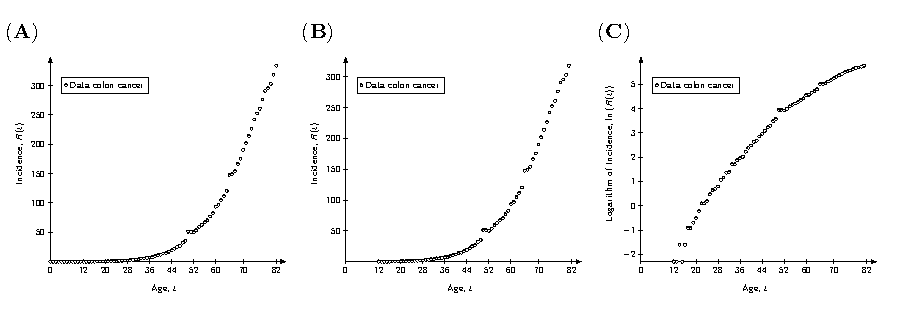
\includegraphics[width=\textwidth]{FigS4.pdf}
  \caption[Processing of the data]{\textit{Processing of the data}. The processing of the original data in (\textbf{A}) is conducted in two steps. (\textbf{B}) Remove all zero incidences corresponding to all ages below 12 years. More precisely, this corresponds to the removal of the first 12 data points in the original time series. (\textbf{C}) Apply the logarithm to the incidences so that $\ln\left(R(t)\right)$ is reported as a function of the age $t$.}
  \label{fig:data_processing}
  \end{figure}

  The logarithmic version of the PLM given by

  $$R(t)=At^{\gamma}$$
  is given by
  $$\ln\left(R(t)\right)=\ln(A)+\gamma\ln(t).$$
  The logarithmic version of the IM-II given by
  $$R(t)=\dfrac{A}{\exp\left(e^{-\alpha(t-\tau)}\right)-1}$$
  is given by
  $$\ln\left(R(t)\right)=\ln(A)-\ln\left(\exp\left(e^{-\alpha(t-\tau)}\right)-1\right).$$
  Again, it is the logarithmic versions of the models that are fitted to the processed data (Fig \ref{fig:data_processing}C).

  To evaluate the fit of the models to the data, the classical \textit{Root Mean Square} (\textit{RMS}) is used as a measure of the fit. Here, the RMS is denoted by $\rho_0$ as in \cite{ohlsson2020symmetry} and it is defined as the square root of a fraction. This fraction defined by a numerator given by the sum of the residuals between the data and the fitted model and a denominator being the number of data points in the time series. The smaller the value of the RMS $\rho_0$ the better the fit of the model to the data. 
  

  